\let\negmedspace\undefined
\let\negthickspace\undefined
\documentclass[journal]{IEEEtran}
\usepackage[a5paper, margin=10mm, onecolumn]{geometry}
%\usepackage{lmodern} % Ensure lmodern is loaded for pdflatex
\usepackage{tfrupee} % Include tfrupee package

\setlength{\headheight}{1cm} % Set the height of the header box
\setlength{\headsep}{0mm}     % Set the distance between the header box and the top of the text

\usepackage{gvv-book}
\usepackage{gvv}
\usepackage{cite}
\usepackage{amsmath,amssymb,amsfonts,amsthm}
\usepackage{algorithmic}
\usepackage{graphicx}
\usepackage{textcomp}
\usepackage{xcolor}
\usepackage{txfonts}
\usepackage{listings}
\usepackage{enumitem}
\usepackage{mathtools}
\usepackage{gensymb}
\usepackage{comment}
\usepackage[breaklinks=true]{hyperref}
\usepackage{tkz-euclide} 
\usepackage{listings}
% \usepackage{gvv}                                        
\def\inputGnumericTable{}                                 
\usepackage[latin1]{inputenc}                                
\usepackage{color}                                            
\usepackage{array}                                            
\usepackage{longtable}                                       
\usepackage{calc}                                             
\usepackage{multirow}                                         
\usepackage{hhline}                                           
\usepackage{ifthen}                                           
\usepackage{lscape}
\begin{document}

\bibliographystyle{IEEEtran}
\vspace{3cm}

\title{4.3.16}
\author{EE25btech11028 - J.Navya sri}
% \maketitle
% \newpage
% \bigskip
{\let\newpage\relax\maketitle}


% Note: \myvec is a custom command often used for column vectors. 
% For this solution, standard 'pmatrix' will be used, but you can define \myvec if needed.
% \newcommand{\myvec}[1]{\begin{pmatrix}#1\end{pmatrix}}


\textbf{Question:} \\
Find the equation of the plane through the points
\[
(2,1,0), \quad (3,-2,-2), \quad (3,1,7).
\]
\textbf{Solution:}
Let $\mathbf{p}_1, \mathbf{p}_2, \mathbf{p}_3$ be the given points and $\mathbf{x} = \begin{pmatrix} x\\y\\z \end{pmatrix}$ be a general point on the plane. The points are:
\[
\mathbf{p}_1 = \begin{pmatrix} 2\\1\\0 \end{pmatrix}, \quad
\mathbf{p}_2 = \begin{pmatrix} 3\\-2\\-2 \end{pmatrix}, \quad % Corrected P_2: (3, -2, -2)
\mathbf{p}_3 = \begin{pmatrix} 3\\1\\7 \end{pmatrix}.
\]
\subsection*{Step 1: General Plane Equation}
The equation of the plane is $\mathbf{n} \cdot \mathbf{x} + d = 0$, where $\mathbf{n} = \begin{pmatrix} a\\b\\c \end{pmatrix}$ is the normal vector.
\[
ax + by + cz + d = 0 \tag{1}
\]
\subsection*{Step 2: Substitution of Points}
The points $\mathbf{p}_i$ must satisfy the plane equation:

\[
2a + b + d = 0 \tag{2}
\]
\[
3a - 2b - 2c + d = 0 \tag{3}
\]
\[
3a + b + 7c + d = 0 \tag{4}
\]
\subsection*{Step 3: Matrix Form}
The system of linear equations can be written as $M \mathbf{v} = \mathbf{0}$, where $\mathbf{v} = \begin{pmatrix} a\\ b\\ c\\ d \end{pmatrix}$:
\[
\begin{pmatrix}
2 & 1 & 0 & 1\\
3 & -2 & -2 & 1\\
3 & 1 & 7 & 1
\end{pmatrix}
\begin{pmatrix} a\\ b\\ c\\ d \end{pmatrix}
=
\begin{pmatrix} 0\\0\\0 \end{pmatrix}
\tag{5}
\]
\subsection*{Step 4: Solving the System}
From (2):
\[
d = -2a - b \tag{6}
\]

Substitute (6) in (3):
\[
3a - 2b - 2c + (-2a - b) = 0 \;\;\Rightarrow\;\; a - 3b - 2c = 0 \tag{7}
\]

Substitute (6) in (4):
\[
3a + b + 7c + (-2a - b) = 0 \;\;\Rightarrow\;\; a + 7c = 0 \tag{8}
\]

From (8):
\[
a = -7c \tag{9}
\]

From (7), substitute (9):
\[
(-7c) - 3b - 2c = 0 \;\;\Rightarrow\;\; -9c = 3b \;\;\Rightarrow\;\; b = -3c \tag{10}
\]

From (6), substitute (9) and (10):
\[
d = -2(-7c) - (-3c) = 14c + 3c \;\;\Rightarrow\;\; d = 17c \tag{11}
\]
{Step 5: Final Result}
The coefficient vector $\mathbf{v}$ is proportional to $c$:
\[
\mathbf{v} = \begin{pmatrix} a\\ b\\ c\\ d \end{pmatrix} = c \begin{pmatrix} -7\\ -3\\ 1\\ 17 \end{pmatrix}
\]

Choosing $c=1$, the normal vector is $\mathbf{n} = \begin{pmatrix} -7\\ -3\\ 1 \end{pmatrix}$ and $d=17$. The plane equation is:
\[
-7x - 3y + z + 17 = 0 \tag{12}
\]

Or equivalently, multiplying by $-1$:
\[
\boxed{7x + 3y - z - 17 = 0} \tag{13}
\]

\begin{figure}[H]
\begin{center}
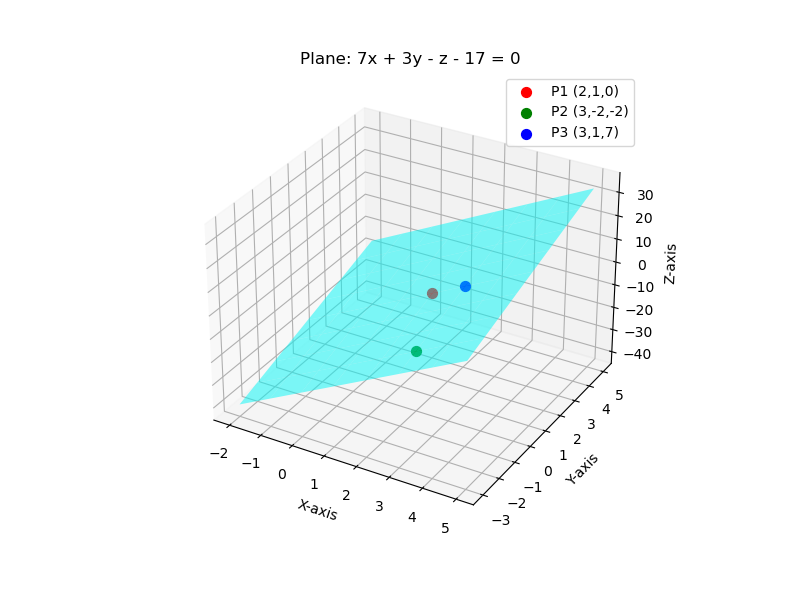
\includegraphics[width=0.6\columnwidth]{figs/fig6.png}
\end{center}
\caption{}
\label{fig:Fig}
\end{figure}


\end{document}